\section{Auswertung}
\label{sec:Auswertung}

\subsection{Abmessung des Acrylblocks} 
Es werden die Abmessungen eines Acrylblocks mit der Schieblehre und durch
einen Amplituden-Scan bestimmt. Die ermittelten Abmessungen mit der Schieblehre
sind \autoref{tab:10} zu entnehmen. Bei der Methode durch den A-Scan wird der 
Acrylblock von oben und unten an der Stelle von jedem Loch gescannt und 
Die Laufzeit des Ultraschalls gemessen. Aus dieser Laufzeit lässt sich durch
\autoref{eqn:2} die Strecke $s$ bis zur Fehlstelle bestimmen. Die Fehlstellen
sind hier die Löcher im Acrylblock. Die Laufzeiten von beiden Seiten sowie die
Umrechnung in die Abstände sind \autoref{tab:11} zu entnehmen. 
\begin{table}[H]
  \centering
  \caption{Abmessungen Schiebleere}
  \label{tab:10}
  \begin{tblr}{
          colspec = {S S S},
          row{1} = {guard, mode = math},
      }
      \toprule
      Loch & d \, \unit{\mm}& y-Position \, \unit{\mm}\\
      \midrule
      1  &   1.55 +- 0.05&   59.05 +- 0.05\\
      2  &   1.55 +- 0.05&   60.8  +- 0.05\\
      3  &   6.05 +- 0.05&   13.15 +- 0.05 \\
      4  &   5    +- 0.05&   21.8  +- 0.05\\
      5  &   4.95 +- 0.05&   30.3  +- 0.05\\
      6  &   3.05 +- 0.05&   38.7  +- 0.05\\
      7  &   3.1  +- 0.05&   46.7  +- 0.05\\
      8  &   3.05 +- 0.05&   54.75 +- 0.05 \\
      9  &   3.1  +- 0.05&   62.7  +- 0.05\\
      10  &  3.1  +- 0.05&   70.7  +- 0.05\\
      11  &  10.0 +- 0.05 &   15.3 +- 0.05 \\
      \bottomrule 
  \end{tblr}
\end{table}
\noindent Um aus der Laufzeit auf den Abstand schließen zu können, muss die
Schallgeschwindigkeit im Medium bekannt sein. Diese wird durch eine lineare 
Regression bestimmt: Dabei wird der mit einer Schieblehre gemessene y-Abstand
der Trennlinie jedes Lochs gegen die zugehörige Laufzeit des Schalls (Hin- und
Rückweg zur Sonde) aufgetragen. Aus der Steigung der Ausgleichsgeraden ergibt
sich die Schallgeschwindigkeit als zurückgelegte Strecke pro Zeiteinheit. Die
Ausgleichsrechnung ist in \autoref{fig:10} dargestellt.
\begin{figure}[H]
  \centering 
  \caption{Lineare Regression zur Bestimmung der Schallgeschwindigkeit im Acrylblock.}
  \label{fig:10}
  \includegraphics{build/plot1.pdf}
\end{figure}
\noindent Die Parameter der Ausgleichsrechnung lauten 
\begin{align}
  m &= \qty{1374(14)}{\meter\per\second}\\
  b &= \qty{-0.0012(0.0004)}{\meter}.
\end{align}
Daraus ergibt sich eine Schallgeschwindigkeit von $v_\text{s,Acryl} = m
\cdot 2 = \qty{2748(28)}{\meter\per\second}$, welche in die Berechnung der
Abmessungen bereits einfließt.

\begin{table}[H]
  \centering
  \caption{Laufzeiten im Acryl und daraus ermittelte Abmessungen.}
  \label{tab:11}
  \begin{tblr}{
          colspec = {S S S S S S},
          row{1} = {guard, mode = math},
      }
      \toprule
      Loch & t_\text{Oben} \, / \unit{\micro\second} 
           & s_\text{Oben} \, / \unit{\mm} 
           & t_\text{Unten} \, / \unit{\micro\second}
           & s_\text{Unten} \, / \unit{\mm}
           & d \, \unit{\mm}\\
      \midrule
      1   & 13.8  & 18.96+-0.19 & 44.0 & 60.5+-0.6   & 1.924+-0.020 \\
      2   & 15.3  & 21.02+-0.21 & 45.1 & 62.0+-0.6   & -1.649+-0.017\\
      3   & 45.1  & 62.0+-0.6   & 10.4 & 14.29+-0.15 & 5.08+-0.05   \\
      4   & 39.7  & 54.5+-0.6   & 16.5 & 22.67+-0.23 & 4.12+-0.04   \\
      5   & 34.0  & 46.7+-0.5   & 23.6 & 32.43+-0.33 & 2.198+-0.022 \\
      6   & 28.6  & 39.3+-0.4   & 29.0 & 39.8+-0.4   & 2.198+-0.022 \\
      7   & 22.6  & 31.05+-0.32 & 34.9 & 48.0+-0.5   & 2.336+-0.024 \\
      8   & 16.8  & 23.08+-0.24 & 40.0 & 55.0+-0.6   & 3.298+-0.034 \\
      9   & 10.9  & 14.98+-0.15 & 46.8 & 64.3+-0.7   & 2.061+-0.021 \\
      10  & 5.1   & 7.01+-0.07  & 0    &  0.0+-0     & -  \\
      11  & 0     & 0.0+-0      & 11.9 & 16.35+-0.17 & -     \\
      \bottomrule
  \end{tblr}
\end{table}

\subsection{Das Auge}
Als Nächstes wird durch analoges Verfahren die Abmessung in einem Auge bestimmt.
\begin{table}[H]
  \centering
  \caption{Abmessungen Schieblehre}
  \label{tab:10}
  \begin{tblr}{
          colspec = {S S S},
          row{1} = {guard, mode = math},
      }
      \toprule
      \text{Part} & t \, / \unit{\micro\second} & \text{Abstand} \, x \, / \unit{\mm}\\
      \midrule
      \text{Iris}          & 11.0 & 15.11+-0.15 \\
      \text{Linseneingang} & 17.0 & 23.36+-0.24 \\
      \text{Linsenausgang} & 24.9 & 34.21+-0.35 \\
      \text{Retina}        & 70.0 & 96.2+-1.0   \\
      \bottomrule 
  \end{tblr}
\end{table}

\subsection{Die Tumore}
Die beiden Tumore im Brustmodell sind in \autoref{fig:11} $\left(T_1\right)$ 
und \autoref{fig:12} $\left(T_2\right)$ abgebidet. Anhand der Bilder wird die
Lage der Tumore bestimmt.
\begin{figure}[H]
  \centering
  \caption{Tumor $T_1$}
  \label{fig:11}
  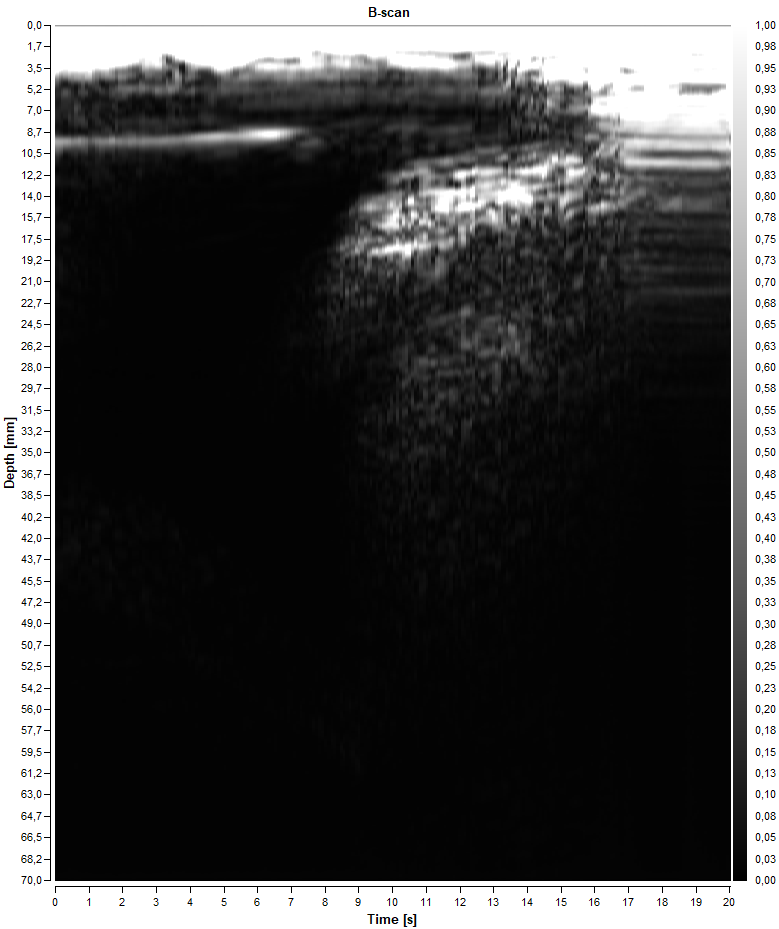
\includegraphics[width=0.8\textwidth]{Bilder/BrustA1.png}
\end{figure}
\noindent Der Tumor in \autoref{fig:11} befindet sich \qty{8.7(1.7)}{\mm} tief
in der Brust und verfügt über einen Durchmesser von \qty{37.5(1.7)}{\mm}.
\begin{figure}[H]
  \centering
  \caption{Tumor $T_2$}
  \label{fig:12}
  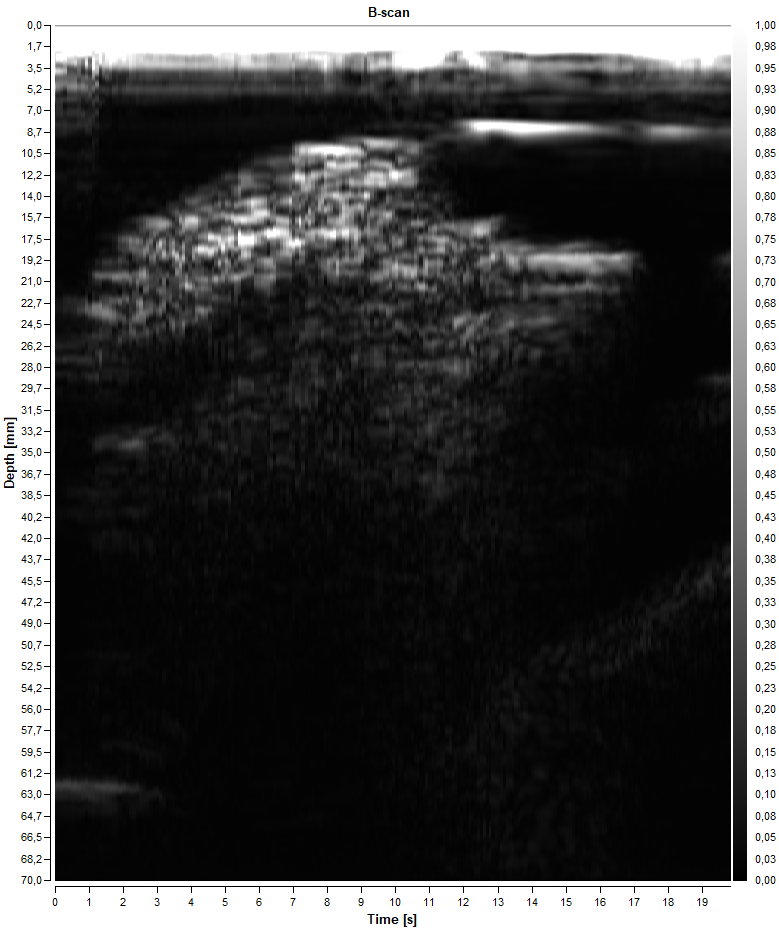
\includegraphics[width=0.8\textwidth]{Bilder/BrustB1.png}
\end{figure}
\noindent Tumor $T_2$ in \autoref{fig:11} befindet sich \qty{8.7(1.7)}{\mm}
tief in der Brust und beläuft sich auf einen Durchmesser von \qty{22.3(1.7)}{\mm}.

%\subsection{Herzmodell}
%\begin{figure}
%  \centering
%  \caption{Tumor $T_1$}
%  \label{fig:13}
%  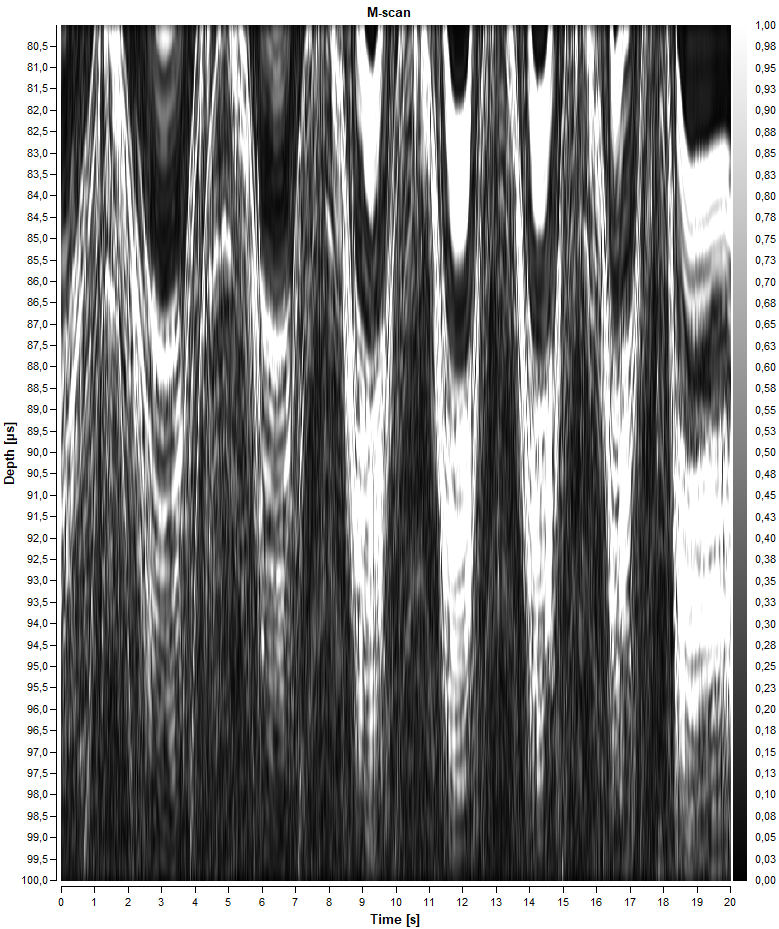
\includegraphics[width=0.5\textwidth]{Bilder/Herz.png}
%\end{figure}
\subsection{Das Herzmodell}

\begin{figure}[H]
  \centering
  \caption{Herzschläge}
  \label{fig:14}
  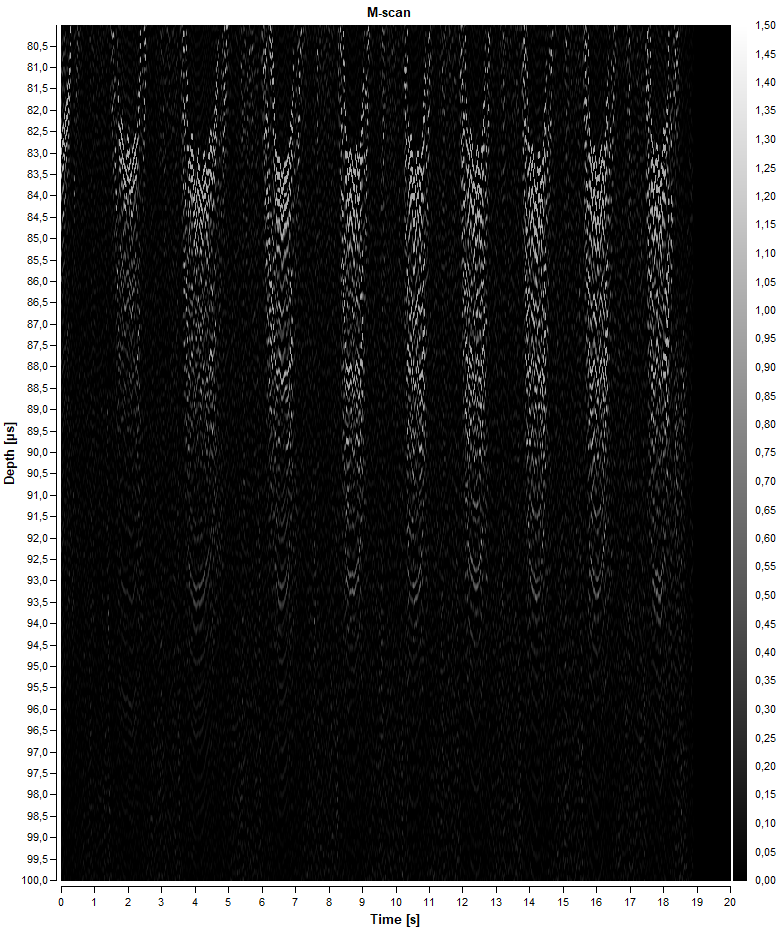
\includegraphics[width=0.8\textwidth]{Bilder/Herz2.png}
\end{figure}

\begin{table}[H]
  \centering
  \caption{Abmessungen Schieblehre.}
  \label{tab:13}
  \begin{tblr}{
          colspec = {S S S},
          row{1} = {guard, mode = math},
      }
      \toprule
      \text{Part} & t \, / \unit{\micro\second}& \text{Abstand} \, x / \unit{\mm}\\
      \midrule
      1 & 1 & 93.5  \\
      2 & 2 & 93.5  \\
      3 & 2 & 93.5   \\
      4 & 1 & 93.5  \\
      5 & 1 & 93.5 \\
      6 & 1 & 93.5  \\
      7 & 1 & 93.5   \\
      8 & 1 & 93.5  \\
      \bottomrule 
  \end{tblr}
\end{table}
\noindent In \autoref{fig:14} sind die Herzschläge aus dem TM-Scan abgebildet. 
Daraus wird graphisch die Breite und Höhe der Schläge abgelesen, in \autoref{tab:13}
eingetragen und der Mittelwert gebildet. In 18 Sekunden schlug das Herz 
neun mal, was einer Herzfrequenz von $v_{Herz} = 0.5$ Schlägen pro Seknde entspricht.
Der endystolische Durchmesser kann durch folgende Formel bestimmt werden 
\begin{equation}
  ESD = \frac{c_\text{wasser} \cdot A}{2}
\end{equation}
A ist dabei die gemittelte Amplitude $\overline{A} = \qty{93.5(0.5)}{}$. Mit
Werten ergibt sich $ ESD = \qty{0.0694(0.0004)}{\meter}$. Daraus ergibt sich
das endystolische Herzvolumen zu 
\begin{equation}
  ESV = \frac{4\cdot \pi}{3}\cdot\left(\frac{ESD}{2}\right)^3 = \qty{0.0001748(0.0000028)}{\meter^3}
\end{equation}
Das Herzschlagvolumen ist damit zu
\begin{equation}
  V_\text{herz} = ESV \cdot v_\text{herz} = \qty{8.74(0.14)e-05}{\meter^3\per\second}
\end{equation}
bestimmt.
